\documentclass{homework}
\usepackage{lipsum}
\usepackage{cancel}
\usepackage{amsthm}
\usepackage{cleveref}
\usepackage{upgreek}
\usepackage[framed]{mcode}
\usepackage{mathrsfs}
\usepackage{tikz}
\usepackage{units}
\usetikzlibrary{matrix}
\newtheorem{lemma}{Lemma}
\DeclareMathOperator*{\argmin}{arg\,min}

\title{Kevin Joyce}
\course{Math 514 - Inverse Problems - Homework 5}
\author{Kevin Joyce}
\docdate{\today}
\begin{document} 
\newcommand{\figref}[1]{\figurename~\ref{#1}}
\renewcommand{\bar}{\overline}
\renewcommand{\hat}{\widehat}
\renewcommand{\SS}{\mathcal S}
\newcommand{\HH}{\mathscr H}
\newcommand{\mom}{\widetilde}
\newcommand{\mle}{\widehat \Uptheta}
\newcommand{\eps}{\varepsilon}
\newcommand{\todist}{\stackrel{D}\longrightarrow}
\newcommand{\toprob}{\stackrel{p}\longrightarrow}
\newcommand{\TTheta}{\overline{\underline \Theta} }
\newcommand{\del}{\partial}
\newcommand{\approxsim}{\overset{\cdotp}{\underset{\cdotp}{\sim}}}

Codes for each problem are available at \url{https://github.com/kjoyce/inverse_problems/tree/master/homework04/codes}

\begin{longproblem}

  \subproblem{Derive the formulas for the UPRE analogous to (3.18) for GCV.  Add lines of code to \texttt{Deblur2dPeriodic.m} so that it implements UPRE.}

  Assuming the derivation from the GCV formulation, we have the following forms for $\|\vect{Ax}_\alpha - \vect b\|^2$ and $\mathrm{tr}(\vect{AA}_\alpha)$,
  $$
    U(\alpha) = \|\vect{Ax}_\alpha - \vect b\|^2 + 2\sigma^2 \mathrm{tr}(\vect{AA_{\alpha}}) = \sum_{i,j}^n \frac{\alpha^2 \vect{\hat B}_{i,j}}{(|\vect{\hat a_s} |^2_{ij} + \alpha)^2}  + 2\sigma^2 \sum_{i,j}^n \frac{|\vect{\hat a_s} |^2_{ij}}{|\vect{\hat a_s} |^2_{ij} + \alpha}.
  $$
  where $\vect{\hat B} = \mathrm{DFT}( \vect B )$ and $\vect{\hat a_s} = n^2 \mathrm{DFT}( \vect{a_s} )$.  The Matlab codes implementing this are as follows:
  \lstinputlisting[language=matlab, firstline=41, lastline=43]{Deblur2dPeriodic.m}

  \subproblem{Derive the formulas for the DP analogous to (3.18) for GCV.  Add lines of code to \texttt{Deblur2dPeriodic.m} so that it implements DP regularization parameter selection methods.}
  Under similar assumptions as above, we obtain
  $$
    D(\alpha) = \|\vect{Ax}_\alpha - \vect b\|^2 - n^2\sigma^2 = \sum_{i,j}^n \frac{\alpha^2 \vect{\hat B_{i,j}}}{(|\vect{\hat a_s} |^2_{ij} + \alpha)^2} - n^2 \sigma^2.
  $$
  The relevant Matlab code is:

  \lstinputlisting[language=matlab, firstline=44, lastline=45]{Deblur2dPeriodic.m}

The reconstructions from these, and the two given parameter selection methods are given in the figure below.

\begin{center}
  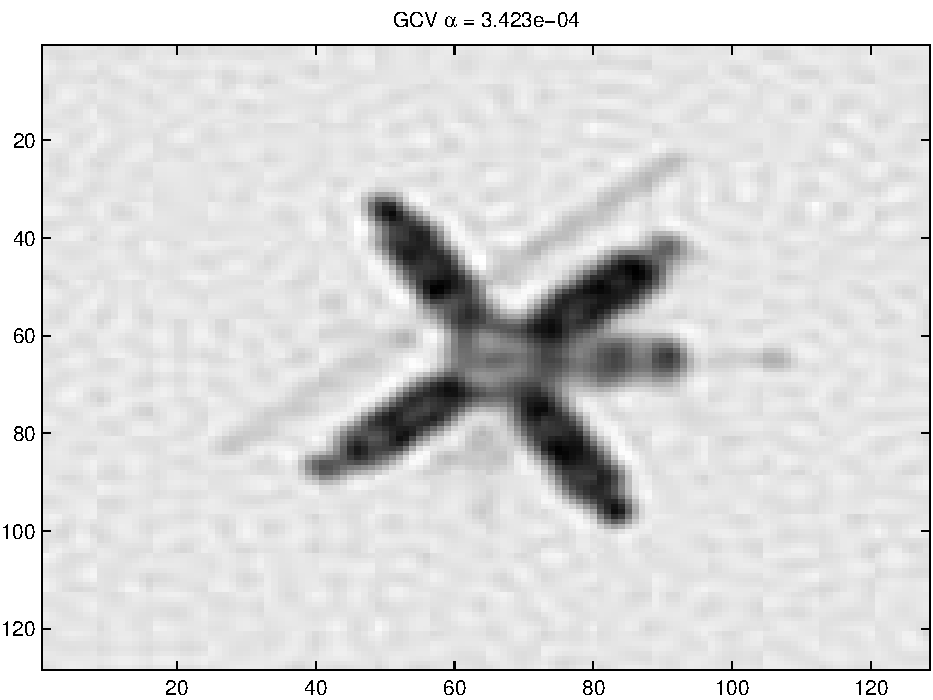
\includegraphics[width=.24\textwidth]{sat_gcv.pdf}
  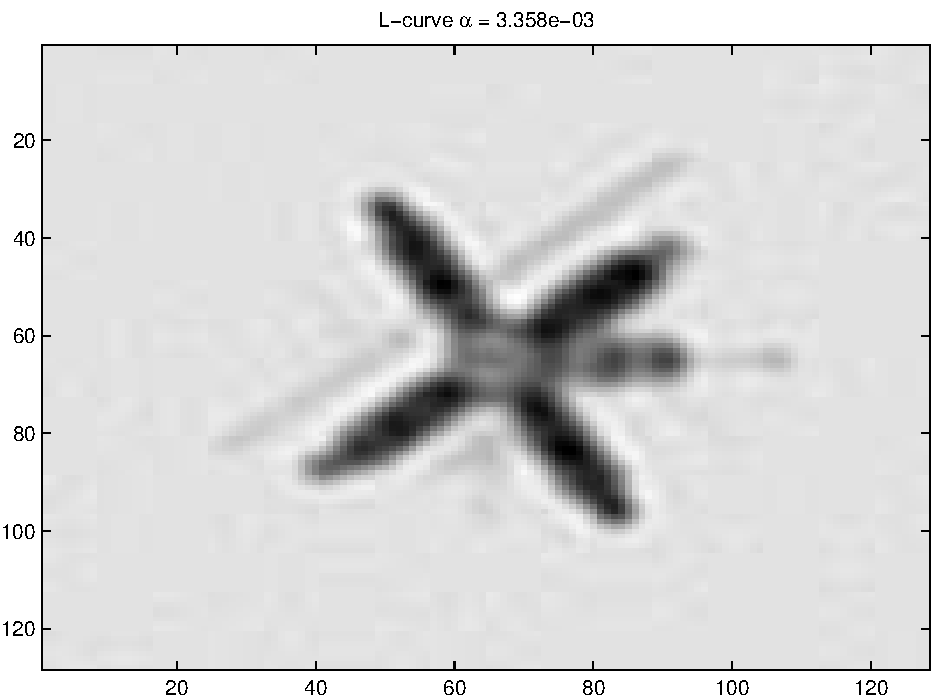
\includegraphics[width=.24\textwidth]{sat_lcv.pdf}
  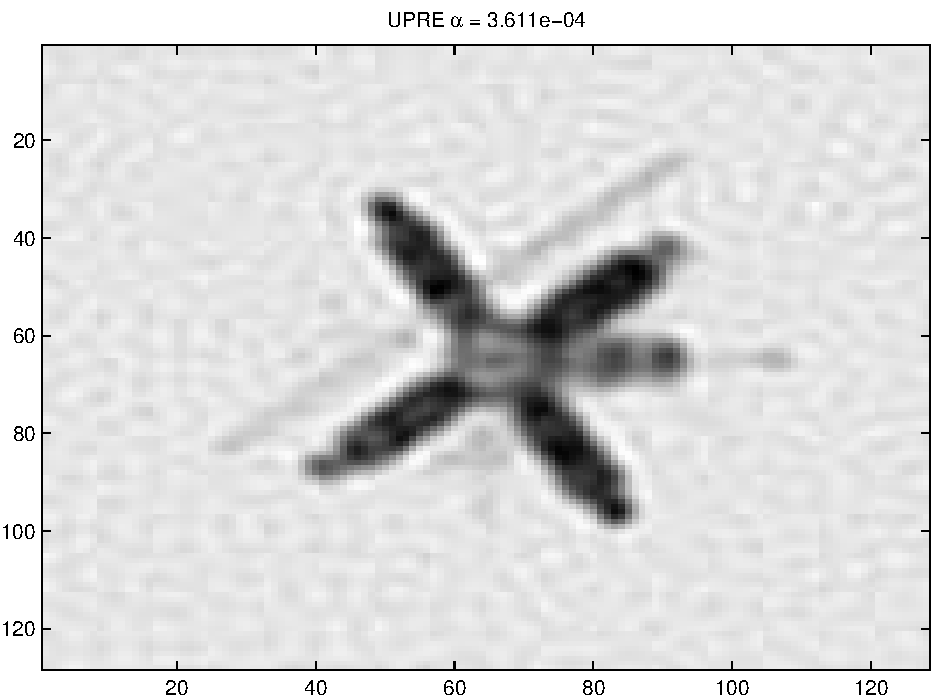
\includegraphics[width=.24\textwidth]{sat_upre.pdf}
  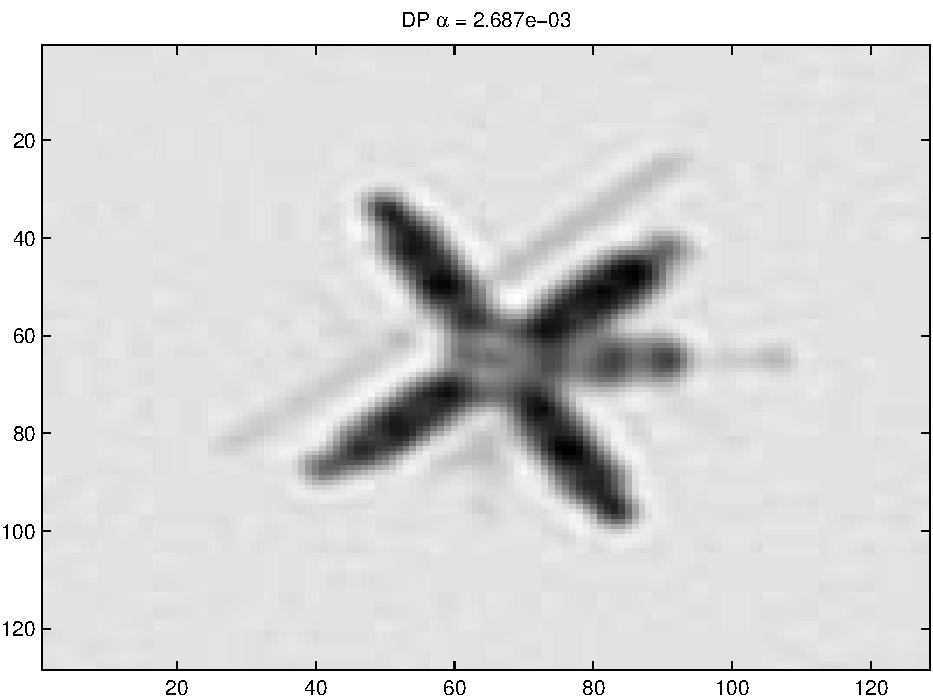
\includegraphics[width=.24\textwidth]{sat_dp.pdf}
\end{center}

\end{longproblem}

\problem{Bardsley 3.11. \emph{An example in which the periodic boundary conditions assumption is poor.} Implement Tikhonov regularization with periodic a boundary condition and GCV stopping rule on the example given in \texttt{PeriodicBCtest.m}.  Note that the blurred image is the central $128\times128$ pixels of a $256\times256$ image and hence does not contain boundary artifacts from the periodic boundary conditions assumed for the forward model.  Perform the deblurring on the $128\times 128$ subimage.  Plot a picture of the deblurred image. } 

\begin{solution}
The relevant codes for implementing this are given below:
  \lstinputlisting[language=matlab, firstline=32, lastline=39]{PeriodicBCtest.m} 

  A plot of the reconstruction is given below.  Note the severe boundary artifacts.
  \begin{center}
    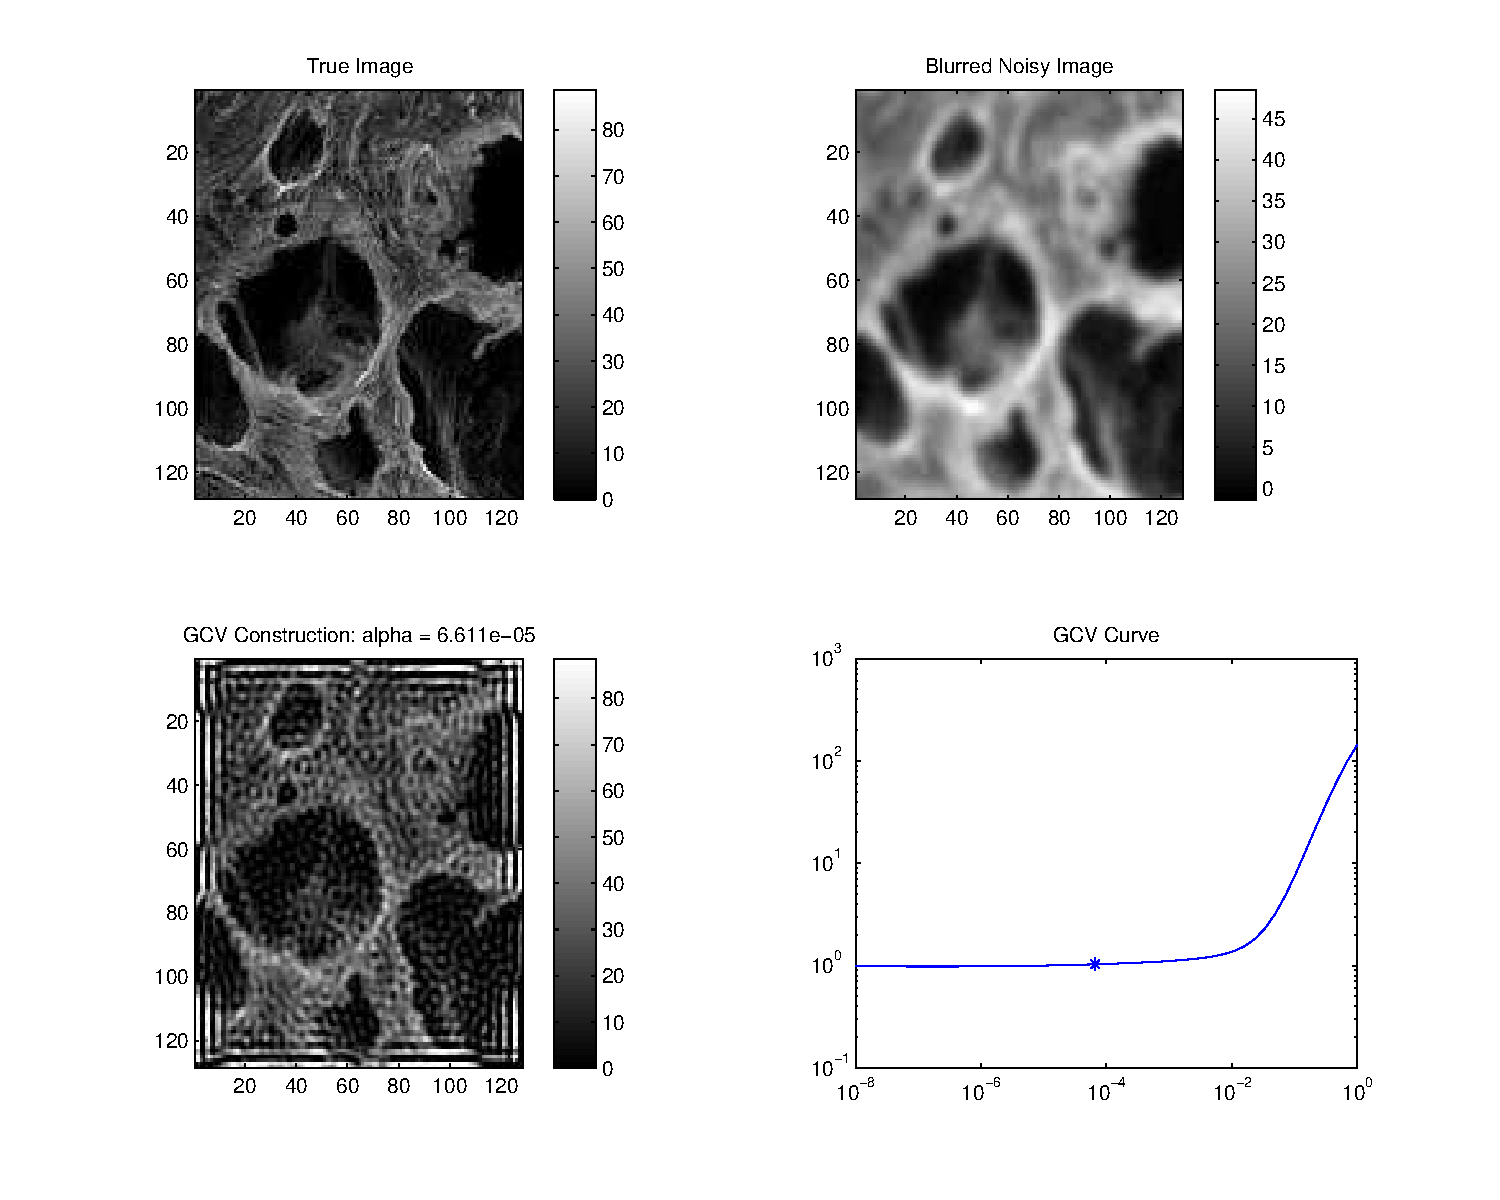
\includegraphics[width=.9\textwidth]{boundary_bad.pdf}
  \end{center}  
\end{solution}

\begin{longproblem}
Modify \texttt{Deblur2DataDriven.m} so that the truncated Landweber iteration, introduced in Chapter 2, is used for solving the deblurring problem.  Use the DP stopping rule, i.e. choose the first $k$ such that $\|\vect{Ax_k} - \vect b\|^2 \le n^2\sigma^2.$
\end{longproblem}

\begin{solution}
  The relevant codes for implementing this are given below.
{\small
\begin{lstlisting}
x = zeros(nx,ny);
tau = .8;% * 1/max(ahat(:));
figure()
n = 0;
while( true )
  n = n+1;
  resid = DA_mult(x,ahat)-b;
  x = x - tau*AtDt_mult(resid,ahat);
  if norm(resid)^2 <= nx*ny*noise^2; break; end; % end if you actually can
  end;
end
\end{lstlisting}

\lstinputlisting[language=matlab]{DA_mult.m}
\lstinputlisting[language=matlab]{AtDt_mult.m}

An image of the resulting reconstruction is given below.
\begin{center}
  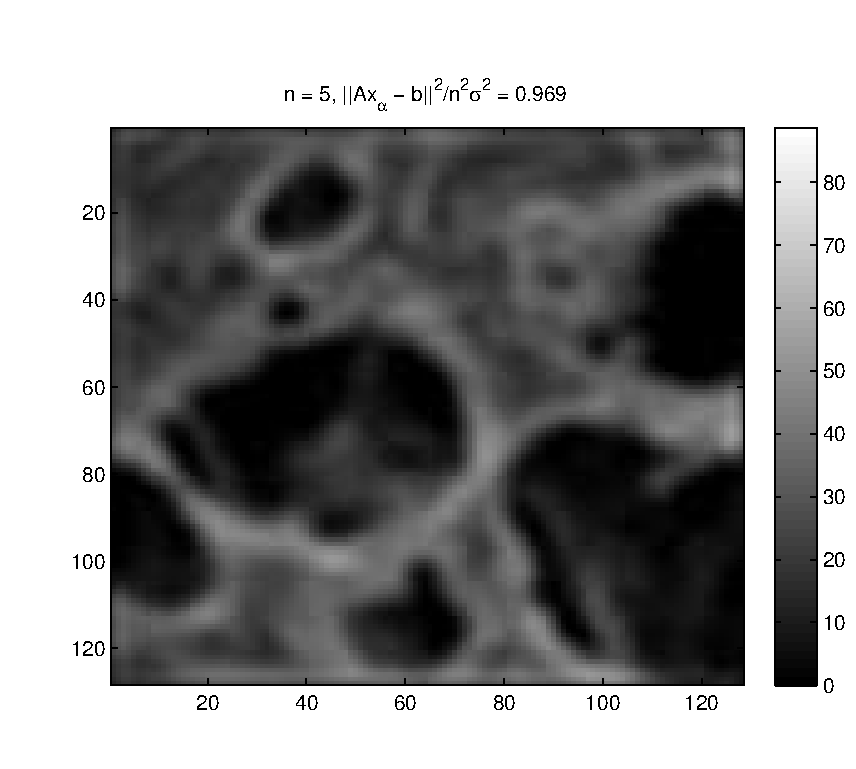
\includegraphics[width=.6\textwidth]{data_driven.pdf}
\end{center}
}
\end{solution}

\end{document} 
